%
% 000-session13.tex
% Presentation Session 13: Practice 4 - Bases Web Server
%
% Compile to .pdf with LaTeX (pdflatex)
% Requires Beamer package (latex-beamer)
%

\documentclass[xcolor=table]{beamer}
\usetheme{Warsaw}
\beamertemplatenavigationsymbolsempty
\setbeamertemplate{headline}{}
\setbeamerfont{title}{size=\large}
\useoutertheme{infolines}
\usepackage[english]{babel}
\usepackage[utf8]{inputenc}
\usepackage{graphics}
\usepackage{amssymb}
\usepackage{multirow}
\usepackage{xcolor}
\usepackage{framed}
\usepackage{hyperref}
\usepackage{tikz}
\usetikzlibrary{arrows.meta, positioning}

\definecolor{shadecolor}{RGB}{180,180,180}
\definecolor{lightgreen}{RGB}{144,238,144}

%%%%%%%%%%%%%%%%%%%%%%%%%%%%%%%%%%%%%%%%%%%%%%%%%%%%%%%%%%%%%%%%
% Python Highlighting
%%%%%%%%%%%%%%%%%%%%%%%%%%%%%%%%%%%%%%%%%%%%%%%%%%%%%%%%%%%%%%%%
\DeclareFixedFont{\ttb}{T1}{txtt}{bx}{n}{10}
\DeclareFixedFont{\ttm}{T1}{txtt}{m}{n}{10}

% Custom colors
\usepackage{color}
\definecolor{deepblue}{rgb}{0,0,0.5}
\definecolor{deepred}{rgb}{0.6,0,0}
\definecolor{deepgreen}{rgb}{0,0.5,0}
\definecolor{grey1}{rgb}{0.5,0.5,0.5}

\usepackage{listings}

% Python style for highlighting
\newcommand\pythonstyle{\lstset{
language=Python,
basicstyle=\ttm\small,
morekeywords={self},
keywordstyle=\ttb\color{deepblue},
emphstyle=\ttb\color{deepred},
stringstyle=\color{deepgreen},
commentstyle=\small\color{grey1}\ttm,
frame=single,
showstringspaces=false
}}

% HTML style for highlighting
\newcommand\htmlstyle{\lstset{
language=HTML,
basicstyle=\ttm\small,
keywordstyle=\ttb\color{deepblue},
stringstyle=\color{deepgreen},
commentstyle=\small\color{grey1}\ttm,
frame=single,
showstringspaces=false
}}

% Python environment
\lstnewenvironment{python}[1][]
{
\pythonstyle
\lstset{#1}
}
{}

% HTML environment
\lstnewenvironment{htmlcode}[1][]
{
\htmlstyle
\lstset{#1}
}
{}

% Python for inline
\newcommand\pythoninline[1]{{\pythonstyle\lstinline!#1!}}

\newcommand{\asignatura}{Session 13: Practice 4 -- Bases Web Server}
\newcommand{\grado}{Programming in Network Environments}
\newcommand{\curso}{2025-2026}

\title[\asignatura]{\asignatura}
\subtitle{\grado}
\author{URJC}
\institute{GSyC}
\date{Course \curso}

\AtBeginSection[]
{
\begin{frame}<beamer>
\begin{center}
{\LARGE \insertsection}
\end{center}
\end{frame}
}

\begin{document}

\frame{
\maketitle
}

\begin{frame}
\frametitle{Contents}
\tableofcontents
\end{frame}

%%%%%%%%%%%%%%%%%%%%%%%%%%%%%%%%%%%%%%%%%%%%%%%%%%%%%%%%%%%%%%%%
%%%%%%%%%%%%%%%%%%%%%%%%%%%%%%%%%%%%%%%%%%%%%%%%%%%%%%%%%%%%%%%%
% SECTION 1: Session 12 Review
%%%%%%%%%%%%%%%%%%%%%%%%%%%%%%%%%%%%%%%%%%%%%%%%%%%%%%%%%%%%%%%%
%%%%%%%%%%%%%%%%%%%%%%%%%%%%%%%%%%%%%%%%%%%%%%%%%%%%%%%%%%%%%%%%

\section{Review: Session 12 -- HTTP Protocol}

\begin{frame}[fragile]
\frametitle{What We Learned in Session 12 (1/2)}

\textbf{HTTP Protocol}: the language between browsers and web servers.

\begin{itemize}
\item \textbf{Request message} (client $\rightarrow$ server):
  \begin{itemize}
  \item Request line: \texttt{GET /path HTTP/1.1}
  \item Headers (Host, User-Agent, ...)
  \item Blank line + Body (usually empty for GET)
  \end{itemize}
\vspace{0.15cm}
\item \textbf{Response message} (server $\rightarrow$ client):
  \begin{itemize}
  \item Status line: \texttt{HTTP/1.1 200 OK}
  \item Headers: \texttt{Content-Type}, \texttt{Content-Length}
  \item Blank line + Body (HTML content)
  \end{itemize}
\vspace{0.15cm}
\item \textbf{Content-Type}: \texttt{text/plain} vs \texttt{text/html}
\item \textbf{Testing}: \texttt{curl 127.0.0.1:8080 -v}
\end{itemize}

\end{frame}

\begin{frame}[fragile]
\frametitle{What We Learned in Session 12 (2/2)}

\textbf{Building an HTTP response} in our server:

\vspace{0.1cm}

\begin{python}
body = "<h1>Hello!</h1>"

status_line = "HTTP/1.1 200 OK\n"
header = "Content-Type: text/html\n"
header += f"Content-Length: {len(body)}\n"

response = status_line + header + "\n" + body
cs.send(response.encode())
\end{python}

\vspace{0.2cm}

\textbf{Key concepts from S12}:
\begin{itemize}
\item Parse the \textbf{request line} to know what the client wants
\item The \textbf{path} in the request tells us which resource to serve
\item The server can read \textbf{HTML files from disk} and send them
\end{itemize}

\end{frame}

%%%%%%%%%%%%%%%%%%%%%%%%%%%%%%%%%%%%%%%%%%%%%%%%%%%%%%%%%%%%%%%%
%%%%%%%%%%%%%%%%%%%%%%%%%%%%%%%%%%%%%%%%%%%%%%%%%%%%%%%%%%%%%%%%
% SECTION 2: Session 13 Overview
%%%%%%%%%%%%%%%%%%%%%%%%%%%%%%%%%%%%%%%%%%%%%%%%%%%%%%%%%%%%%%%%
%%%%%%%%%%%%%%%%%%%%%%%%%%%%%%%%%%%%%%%%%%%%%%%%%%%%%%%%%%%%%%%%

\section{Session 13: Practice 4 -- Bases Web Server}

\begin{frame}
\frametitle{Session 13 Goals}

\textbf{In this session we will}:

\begin{itemize}
\item Build a \textbf{web server} that serves information about the \textbf{four DNA bases}: A, C, G, T
\item Each base has its own \textbf{HTML page} with a different color
\item Practice writing \textbf{HTML} and serving \textbf{different resources}
\item Handle \textbf{error pages} for unknown resources
\end{itemize}

\vspace{0.4cm}

\textbf{Time}: 2 hours

\vspace{0.2cm}

\textbf{Folder}: \texttt{P04/} with subfolders \texttt{html/info/} and \texttt{html/}

\vspace{0.2cm}

\textbf{Important}: Finish all S12 exercises before starting!

\end{frame}

\begin{frame}
\frametitle{The DNA Bases Web Server: Resources}

Each base has its own page with: \textbf{name}, \textbf{letter}, \textbf{chemical formula}, and a \textbf{link to Wikipedia}.

\vspace{0.2cm}

\begingroup\small
\begin{center}
\begin{tabular}{|l|l|l|}
\hline
\textbf{Resource (path)} & \textbf{HTML File} & \textbf{Color} \\
\hline
\texttt{/info/A} & \texttt{A.html} & lightgreen \\
\hline
\texttt{/info/C} & \texttt{C.html} & yellow \\
\hline
\texttt{/info/G} & \texttt{G.html} & lightblue \\
\hline
\texttt{/info/T} & \texttt{T.html} & pink \\
\hline
\texttt{/} & \texttt{index.html} & white \\
\hline
any other & \texttt{error.html} & red \\
\hline
\end{tabular}
\end{center}
\endgroup

\vspace{0.2cm}

The server is built \textbf{incrementally} -- one or two resources per exercise.

\end{frame}

\begin{frame}
\frametitle{Exercise 1: A.html}

\textbf{Filename}: \texttt{P04/html/info/A.html} -- Write the HTML page for \textbf{Adenine} (template for the others).

\vspace{0.1cm}

\begin{center}
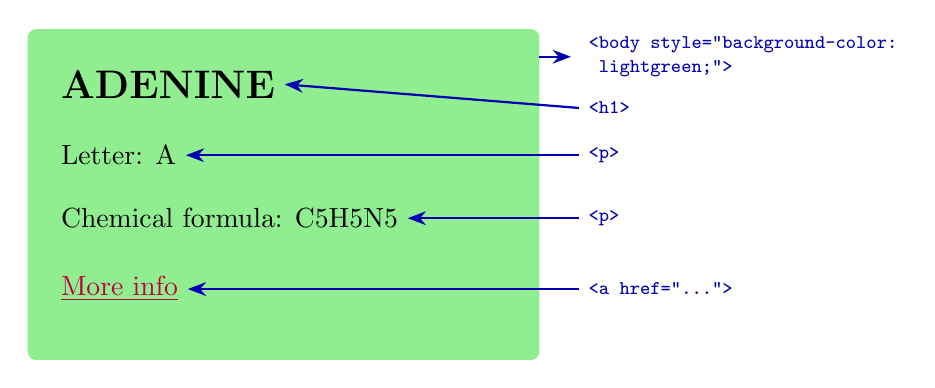
\begin{tikzpicture}
% Green background box
\fill[lightgreen, rounded corners=3pt] (0,0) rectangle (6.5,4.2);

% Content
\node[anchor=west, font=\bfseries\Large] (h1) at (0.3, 3.5) {ADENINE};
\node[anchor=west, font=\normalsize] (p1) at (0.3, 2.6) {Letter: A};
\node[anchor=west, font=\normalsize] (p2) at (0.3, 1.8) {Chemical formula: C5H5N5};
\node[anchor=west, font=\normalsize, text=purple] (link) at (0.3, 0.9) {\underline{More info}};

% Annotations with arrows
\node[anchor=west, font=\scriptsize\ttfamily, text=blue!70!black] (tag0) at (7.0, 4.0) {<body style="background-color:};
\node[anchor=west, font=\scriptsize\ttfamily, text=blue!70!black] at (7.0, 3.7) {~lightgreen;">};
\draw[-{Stealth}, blue!70!black, thick] (6.5, 3.85) -- (6.9, 3.85);

\node[anchor=west, font=\scriptsize\ttfamily, text=blue!70!black] (tag1) at (7.0, 3.2) {<h1>};
\draw[-{Stealth}, blue!70!black, thick] (tag1.west) -- (h1.east);

\node[anchor=west, font=\scriptsize\ttfamily, text=blue!70!black] (tag2) at (7.0, 2.6) {<p>};
\draw[-{Stealth}, blue!70!black, thick] (tag2.west) -- (p1.east);

\node[anchor=west, font=\scriptsize\ttfamily, text=blue!70!black] (tag3) at (7.0, 1.8) {<p>};
\draw[-{Stealth}, blue!70!black, thick] (tag3.west) -- (p2.east);

\node[anchor=west, font=\scriptsize\ttfamily, text=blue!70!black] (tag4) at (7.0, 0.9) {<a href="...">};
\draw[-{Stealth}, blue!70!black, thick] (tag4.west) -- (link.east);
\end{tikzpicture}
\end{center}

\vspace{0.1cm}

\textbf{Preview}: Open the HTML file in PyCharm and click on the browser icon.

\end{frame}

\begin{frame}[fragile]
\frametitle{Exercises 2--3: Serving A and C}

\textbf{Exercise 2}: \texttt{P04/e2.py} -- Serve the A base
\begin{itemize}
\item Web server returns \texttt{A.html} when \texttt{/info/A} is requested
\item For any other resource, send a \textbf{blank body}
\item Parse the request line to extract the \textbf{path}
\end{itemize}

\vspace{0.1cm}

\begin{python}
req_line = lines[0]  # "GET /info/A HTTP/1.1"
parts = req_line.split(" ")
path = parts[1]      # "/info/A"
\end{python}

\vspace{0.2cm}

\textbf{Exercise 3}: \texttt{P04/html/info/C.html} + \texttt{P04/e3.py}
\begin{itemize}
\item Create C.html (yellow background, Cytosine info)
\item Extend the server to also serve \texttt{/info/C}
\item Test: \texttt{http://127.0.0.1:8080/info/C}
\end{itemize}

\end{frame}

\begin{frame}
\frametitle{Exercises 4--5: All Bases + Error Page}

\textbf{Exercise 4}: \texttt{G.html}, \texttt{T.html} + \texttt{P04/e4.py}
\begin{itemize}
\item Create \texttt{G.html} (lightblue) and \texttt{T.html} (pink)
\item Extend the server to serve \texttt{/info/G} and \texttt{/info/T}
\item The server now handles all four DNA bases
\end{itemize}

\vspace{0.4cm}

\textbf{Exercise 5}: \texttt{P04/html/error.html} + \texttt{P04/e5.py}
\begin{itemize}
\item Create an \textbf{error page} with a \textbf{red background}
\item If the user requests \textbf{any resource not implemented}, show the error page
\item Test: \texttt{http://127.0.0.1:8080/whatever}
\end{itemize}

\end{frame}

\begin{frame}
\frametitle{Exercise 6 and Deliverables}

\textbf{Exercise 6}: \texttt{P04/html/index.html} + \texttt{P04/webserver.py}
\begin{itemize}
\item Create an \textbf{index page} (white background) with \textbf{links} to all four bases
\item Served when the user accesses \texttt{/} (the root)
\item Add a \textbf{link back to the main page} in all other HTML files
\item Final version: \texttt{webserver.py}
\end{itemize}

\vspace{0.3cm}

\textbf{P04 folder should contain}:

\begingroup\small
\begin{itemize}
\item \texttt{html/info/A.html}, \texttt{C.html}, \texttt{G.html}, \texttt{T.html}
\item \texttt{html/error.html}, \texttt{html/index.html}
\item \texttt{e2.py}, \texttt{e3.py}, \texttt{e4.py}, \texttt{e5.py}, \texttt{webserver.py}
\end{itemize}
\endgroup

\vspace{0.2cm}

\textbf{Remember}: Push everything to your remote Github repo!

\end{frame}

%%%%%%%%%%%%%%%%%%%%%%%%%%%%%%%%%%%%%%%%%%%%%%%%%%%%%%%%%%%%%%%%
%%%%%%%%%%%%%%%%%%%%%%%%%%%%%%%%%%%%%%%%%%%%%%%%%%%%%%%%%%%%%%%%
% SECTION 3: End
%%%%%%%%%%%%%%%%%%%%%%%%%%%%%%%%%%%%%%%%%%%%%%%%%%%%%%%%%%%%%%%%
%%%%%%%%%%%%%%%%%%%%%%%%%%%%%%%%%%%%%%%%%%%%%%%%%%%%%%%%%%%%%%%%

\begin{frame}
\begin{center}
\Huge{Questions?}

\vspace{1cm}

\Large{Time to code!}
\end{center}
\end{frame}

\end{document}
